\documentclass[12pt]{article}
\usepackage[left=2.5cm,top=2.5cm,right=2.5cm,bottom=2.5cm]{geometry} 
\usepackage{graphicx}
\usepackage[utf8]{inputenc}
\usepackage[T1]{fontenc}
\usepackage{lmodern}
\usepackage{float}
 \usepackage{enumerate}
\usepackage{afterpage}
\usepackage{parskip}
\usepackage{graphicx}
\usepackage{xcolor}
\usepackage[nottoc]{tocbibind}
\usepackage{vmargin}
 \usepackage{amsmath}
\usepackage{amsmath}
\usepackage{algorithm}
\usepackage[noend]{algpseudocode}
\usepackage{tabto}
\usepackage[spanish,english]{babel}
\usepackage{fixltx2e}
\usepackage{enumitem}
\usepackage{amssymb}
\usepackage{color}   %May be necessary if you want to color links
\usepackage{hyperref}
\usepackage{xcolor}
\usepackage[normalem]{ulem}
\renewcommand{\algorithmicforall}{\textbf{for each}}

\definecolor{violetaperlado}{RGB}{40, 114, 51}

\hypersetup{
    colorlinks=true, %set true if you want colored links
    linktoc=all,     %set to all if you want both sections and subsections linked
    linkcolor=violetaperlado,  %choose some color if you want links to stand out
}

\begin{document}
 \setlength\parindent{24pt}
%titlepage
\thispagestyle{empty}
\begin{center}
\begin{minipage}{0.75\linewidth}
    \centering
%University logo
    
\includegraphics[width=0.4\linewidth]{imgs/logo-uclm.jpg}\par
    %\rule{0.4\linewidth}{0.15\linewidth}\par
    \vspace{3cm}
%Thesis title
    {\uppercase{\Large ARM v8 Family Processors\par}}
    \vspace{3cm}
%Author's name
    {\Large Silvia González Rodríguez\par}
    {\Large Miguel Enrique Játiva Jiménez\par}
    {\Large Miguel Sánchez de la Rosa\par}
    \vspace{3cm}
%Degree
    {\Large Computer Architecture\par}
    \vspace{3cm}
%Date
    {\Large December 2019}
\end{minipage}
\end{center}
\clearpage

\pagenumbering{Roman}
\setcounter{page}{2}
\tableofcontents % indice de contenidos

\cleardoublepage
\listoffigures % indice de figuras

\cleardoublepage
\listoftables % indice de tablas
\cleardoublepage

\pagenumbering{arabic} % para empezar la numeración con números

%Introduction
\section{Historic Context}
\hspace{\parindent} ARM, previously Advanced RISC Machine, originally Acorn RISC Machine, is a family of reduced instruction set computing (RISC) architectures for computer processors, configured for various environments. Arm Holdings develops the architecture and licenses it to other companies, who design their own products that implement one of those architectures including systems on chips (SoC) and systems on modules (SoM) that incorporate memory, interfaces, radios, etc. It also designs cores that implement this instruction set and licenses these designs to a number of companies that incorporate those core desings into their own products.\cite{wikipediaintro}\par

The British computer manufacturer Acorn Computers first developed the Acorn RISC Machine architecture (ARM) in the 1980s to use in its personal computers. Its first ARM-based products were coprocessor modules for the BBC Micro series of computers. After the successful BBC Micro computer, Acorn Computers considered how to move on from the relatively simple MOS Technology 6502 processor to address business markets like the one that was soon dominated by the IBM PC, launched in 1981. The Acorn Business Computer (ABC) plan required that a number of second processors be made to work with the BBC Micro platform, but processors such as the Motorola 68000 and National Semiconductor 32016 were considered unsuitable, and the 6502 was not powerful enough for a graphics-based user interface.\cite{wikipediaintro}\par

The official Acorn RISC Machine project started in October 1983. They chose VLSI Technology as the silicon partner, as they were a source of ROMs and custom chips for Acorn. Wilson and Furber led the design. They implemented it with a similar efficiency ethos as the 6502. A key design goal was achieving low-latency input/output (interrupt) handling like the 6502. The 6502's memory access architecture had let developers produce fast machines without costly direct memory access (DMA) hardware. The first samples of ARM silicon worked properly when first received and tested on 26 April 1985.\cite{wikipediaintro}\par

The ARM2 featured a 32-bit data bus, 26-bit address space and 27 32-bit registers. Eight bits from the program counter register were available for other purposes; the top six bits (available because of the 26-bit address space) served as status flags, and the bottom two bits (available because the program counter was always word-aligned) were used for setting modes. The address bus was extended to 32 bits in the ARM6, but program code still had to lie within the first 64 MB of memory in 26-bit compatibility mode, due to the reserved bits for the status flags. The ARM2 had a transistor count of just 30,000, compared to Motorola's six-year-older 68000 model with around 40,000. Much of this simplicity came from the lack of microcode (which represents about one-quarter to one-third of the 68000) and from (like most CPUs of the day) not including any cache. This simplicity enabled low power consumption, yet better performance than the Intel 80286. A successor, ARM3, was produced with a 4 KB cache, which further improved performance.\cite{wikipediaintro}\par

In the late 1980s, Apple Computer and VLSI Technology started working with Acorn on newer versions of the ARM core. In 1990, Acorn spun off the design team into a new company named Advanced RISC Machines Ltd., which became ARM Ltd when its parent company, Arm Holdings plc, floated on the London Stock Exchange and NASDAQ in 1998. The new Apple-ARM work would eventually evolve into the ARM6, first released in early 1992. Apple used the ARM6-based ARM610 as the basis for their Apple Newton PDA.\cite{wikipediaintro}\par

In 1994, Acorn used the ARM610 as the main central processing unit (CPU) in their RiscPC computers. DEC licensed the ARMv4 architecture and produced the StrongARM. At 233 MHz, this CPU drew only one watt (newer versions draw far less). This work was later passed to Intel as part of a lawsuit settlement, and Intel took the opportunity to supplement their i960 line with the StrongARM. Intel later developed its own high performance implementation named XScale, which it has since sold to Marvell. Transistor count of the ARM core remained essentially the same throughout these changes; ARM2 had 30,000 transistors, while ARM6 grew only to 35,000.\cite{wikipediaintro}\par

In 2005, about 98\% of all mobile phones sold used at least one ARM processor. In 2010, producers of chips based on ARM architectures reported shipments of 6.1 billion ARM-based processors, representing 95\% of smartphones, 35\% of digital televisions and set-top boxes and 10\% of mobile computers. In 2011, the 32-bit ARM architecture was the most widely used architecture in mobile devices and the most popular 32-bit one in embedded systems. In 2013, 10 billion were produced and "ARM-based chips are found in nearly 60 percent of the world’s mobile devices".\cite{wikipediaintro}\par



%General characteristics
\section{General characteristics}
\hspace{\parindent} The ARM Cortex-A72 is a microarchitecture implementing the ARMv8-A 64-bit instruction set designed by ARM Holdings' Austin design centre. The Cortex-A72 is a 3-wide decode out-of-order superscalar pipeline. It is available as SIP core to licensees, and its design makes it suitable for integration with other SIP cores (e.g. GPU, display controller, DSP, image processor, etc.) into one die constituting a system on a chip (SoC). The Cortex-A72 was announced in 2015 to serve as the successor of the Cortex-A57, and was designed to use 20\% less power or offer 90\% greater performance. It has one to four cores in a single processor device with L1 and L2 cache subsystems.\cite{cortexA72manual} The following figure \ref{cortexA72conf} shows an example block diagram of a Cortex-A72 processor configuration with four cores.

\begin{figure}[H]
\begin{center}
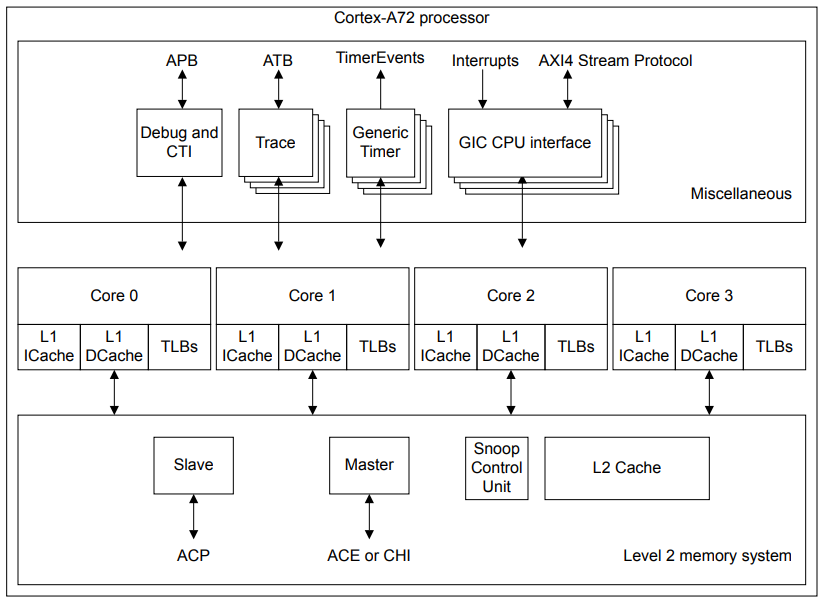
\includegraphics[width=0.8\linewidth]{imgs/foto1.png}
\caption{Example Cortex-A72 processor configuration}
\label{cortexA72conf}
\end{center}
\end{figure}

The Cortex-A72 boasts up to a 50 percent energy reduction when compared with the Cortex-A15 and a 20 percent saving compared with the A57, at the same clock speeds. Milliwatts per core have dropped from the A57, to around 700mW at 2.5GHz.\cite{androidauthority} The design takes up 10 percent less area than the A57, which will also help save on costs. We can see this in figure \ref{cortexA72performance}.

\begin{figure}[H]
\begin{center}
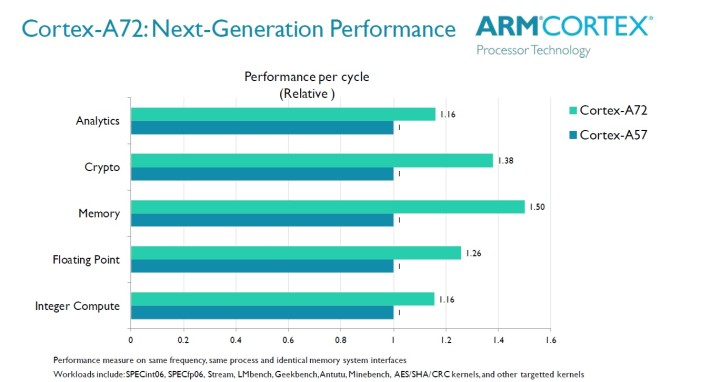
\includegraphics[width=0.8\linewidth]{imgs/foto2.jpg}
\caption{Cortex-A72 performance}
\label{cortexA72performance}
\end{center}
\end{figure}

As well as substantial energy savings, ARM reckons that the A72 will be able to sustain 2.5GHz clocks on the new 16nm process, whilst keeping within the limited smartphone power budget as seen in figure \ref{cortexA72power}. It’s the additional power efficiency and resulting lower heat profile that will really help the A72 achieve higher clock speeds than a 16nm A57.\cite{androidauthority}

\begin{figure}[H]
\begin{center}
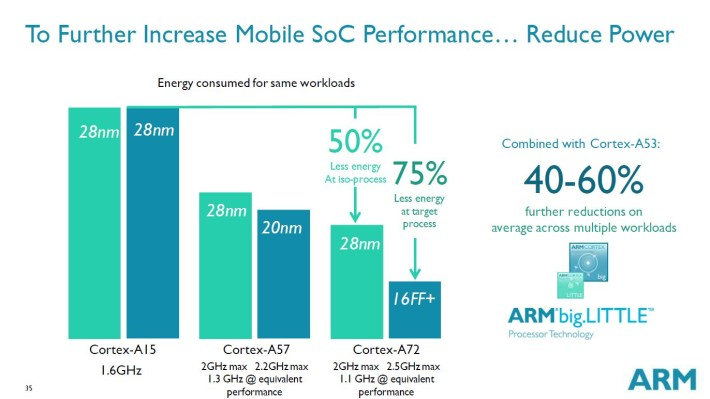
\includegraphics[width=0.8\linewidth]{imgs/foto3.jpg}
\caption{Cortex-A72 power reduction}
\label{cortexA72power}
\end{center}
\end{figure}

ARM is looking to differentiate its high performing designs from their lower energy counterparts. The A53 and A57 are quite different in their design and intended applications, so switching the more powerful cores over to the A7x naming scheme should help avoid any confusion in the future.\cite{androidauthority}

\begin{figure}[H]
\begin{center}
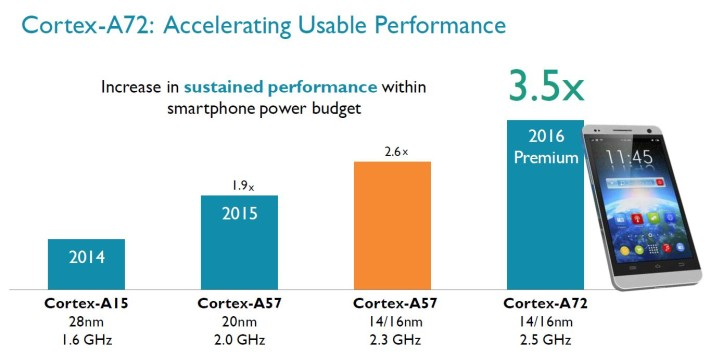
\includegraphics[width=0.8\linewidth]{imgs/foto4.jpg}
\caption{Cortex-A72 usable performance}
\label{cortexA72usable}
\end{center}
\end{figure}

The key point to take-away is that ARM has focused heavily on improving power and area efficiency with the A72, which is always welcome in mobile products. This also has the added benefit of allowing the chip to run cooler and to be clocked slightly higher than its predecessor.\cite{androidauthority}

%Architectural characteristics
\section{Architectural characteristics}

%Bibliografia
\begin{thebibliography}{9}
\bibitem{wikipediaintro} 
Wikipedia.
\textit{ARM architecture}. 

 
\bibitem{cortexA72manual} 
\textit{ARM® Cortex®-A72 MPCore Processor Technical Reference Manual}.

 
\bibitem{androidauthority} 
Robert Triggs. \textit{A closer look at the ARM Cortex-A72}.

\end{thebibliography}




\end{document}